\XtoCBlock{D}
\label{block:D}
\begin{figure}[H]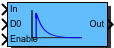
\includegraphics{D}\end{figure} 

\begin{XtoCtabular}{Inports}
In & Control error input\tabularnewline
\hline
D0 & Derivational value which is loaded during initialization.

(Usually this inport is connect to the In inport.)\tabularnewline
\hline
Enable & Enable == 0: Deactivation of block; Out set to 0

Enable 0->1: Preload of derivational part

Enable == 1: Activation of block\tabularnewline
\hline
\end{XtoCtabular}


\begin{XtoCtabular}{Outports}
Out & Control value\tabularnewline
\hline
\end{XtoCtabular}

\begin{XtoCMaskParamTabular}{Mask Parameters}
\rowcolor[gray]{0.8}\textbf{Name} & \textbf{ID} & \textbf{Description}\tabularnewline\hline
Kd & 1 & Derivative Factor\tabularnewline
\hline
fc & 2 & Cutoff frequency of realization low pass\tabularnewline
\hline
ts\_fact & 3 & Multiplication factor of base sampling time (in integer format)\tabularnewline
\hline
\end{XtoCMaskParamTabular}

\subsubsection*{Description:}
D Controller:

    G(s) = Kd*s/(s/(2*pi*fc) + 1)

% include optional documentation file
\InputIfFileExists{\XcHomePath/Library/Control/Doc/D_Info.tex}{\vspace{1ex}}{}

\subsubsection*{Implementations:}
\begin{tabular}{l l}
\textbf{FiP16} & 16 Bit Fixed Point Implementation\tabularnewline
\textbf{FiP32} & 32 Bit Fixed Point Implementation\tabularnewline
\textbf{Float32} & 32 Bit Floating Point Implementation\tabularnewline
\textbf{Float64} & 64 Bit Floating Point Implementation\tabularnewline
\end{tabular}

\XtoCImplementation{FiP16}
\nopagebreak[0]

16 Bit Fixed Point Implementation

\begin{XtoCtabular}{Inports Data Type}
In & int16\tabularnewline
\hline
D0 & int16\tabularnewline
\hline
Enable & bool\tabularnewline
\hline
\end{XtoCtabular}

\begin{XtoCtabular}{Outports Data Type}
Out & int16\tabularnewline
\hline
\end{XtoCtabular}

\ifdefined \AddTestReports
\InputIfFileExists{\XcHomePath/Library/Control/Doc/Test-Results/Test_D_FiP16.tex}{}{}
\fi
\XtoCImplementation{FiP32}
\nopagebreak[0]

32 Bit Fixed Point Implementation

\begin{XtoCtabular}{Inports Data Type}
In & int32\tabularnewline
\hline
D0 & int16\tabularnewline
\hline
Enable & bool\tabularnewline
\hline
\end{XtoCtabular}

\begin{XtoCtabular}{Outports Data Type}
Out & int32\tabularnewline
\hline
\end{XtoCtabular}

\ifdefined \AddTestReports
\InputIfFileExists{\XcHomePath/Library/Control/Doc/Test-Results/Test_D_FiP32.tex}{}{}
\fi
\XtoCImplementation{Float32}
\nopagebreak[0]

32 Bit Floating Point Implementation

\begin{XtoCtabular}{Inports Data Type}
In & float32\tabularnewline
\hline
D0 & int16\tabularnewline
\hline
Enable & bool\tabularnewline
\hline
\end{XtoCtabular}

\begin{XtoCtabular}{Outports Data Type}
Out & float32\tabularnewline
\hline
\end{XtoCtabular}

\ifdefined \AddTestReports
\InputIfFileExists{\XcHomePath/Library/Control/Doc/Test-Results/Test_D_Float32.tex}{}{}
\fi
\XtoCImplementation{Float64}
\nopagebreak[0]

64 Bit Floating Point Implementation

\begin{XtoCtabular}{Inports Data Type}
In & float64\tabularnewline
\hline
D0 & int16\tabularnewline
\hline
Enable & bool\tabularnewline
\hline
\end{XtoCtabular}

\begin{XtoCtabular}{Outports Data Type}
Out & float64\tabularnewline
\hline
\end{XtoCtabular}

\ifdefined \AddTestReports
\InputIfFileExists{\XcHomePath/Library/Control/Doc/Test-Results/Test_D_Float64.tex}{}{}
\fi
